% ------------- recapProtocoleEtudeSeuil -------------
\begin{figure}[htb!] 
\centering
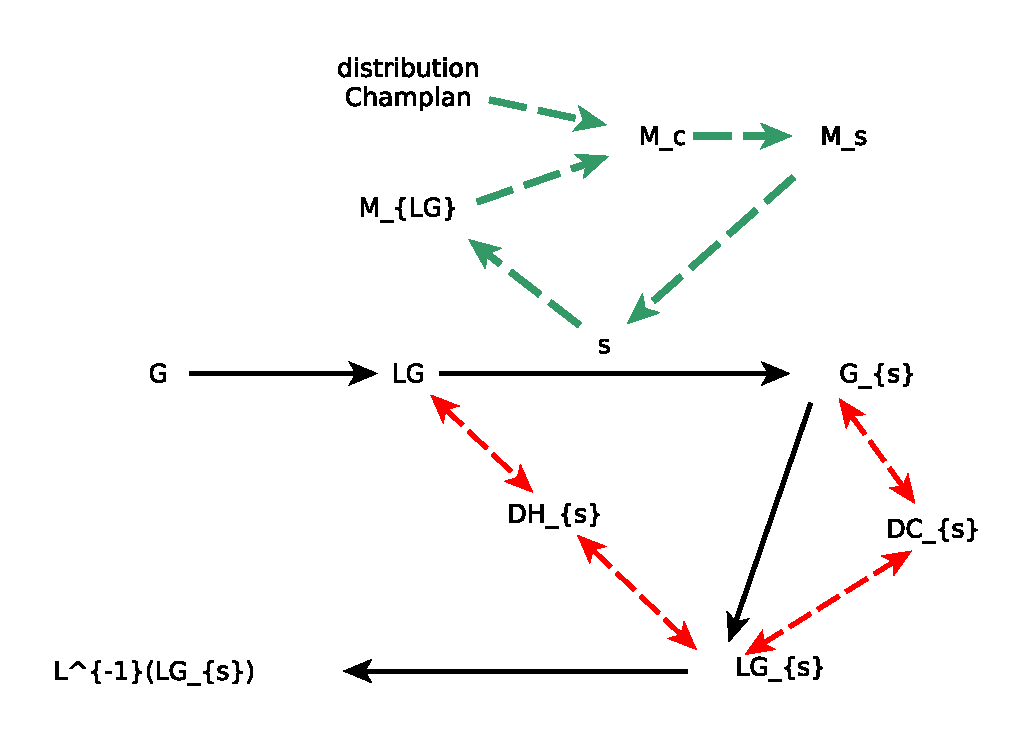
\includegraphics[scale=0.750]{recapProtocoleEtudeSeuil.eps}
\caption{\'Etapes de l'exp\'erimentation :  
1) on g\'en\`ere le graphe $G$ et son line-graphe $LG$, 
2) on  g\'en\`ere la matrice de corr\'elation $M_c$ du line-graphe $LG$   \`a partir de la distribution des valeurs de corr\'elation du graphe de Champlan puis on lui applique une valeur de seuil $s$ pour obtenir le graphe $G_{s}$, 
3) on applique les algorithmes de d\'ecouverte et de correction pour avoir un line-graphe $LG_{s}$. $LG_{s}$ et  $G_{s}$ diff\`erent de $DC_{s}$ ar\^etes. $LG_{s}$ a $DH_{s}$ cases modifi\'ees par rapport \`a $LG$.
}
\label{recapProtocoleEtudeSeuil} 
\end{figure}
% FloatBarrier
% ------------- recapProtocoleEtudeSeuil -------------

Le but de notre couple d'algorithmes est de corriger les cases erron\'ees dans $M_s$ afin que la matrice propos\'ee $M'_{s}$ soit la matrice d'adjacence d'un line-graphe $LG_s$ et que la distance de Hamming entre $LG_s$ et $LG$ soit minimale. 
Pour ce faire, nous recherchons la valeur du seuil $s$ qui mininise la distance de Hamming entre $LG_s$ et $LG$.
\newline

Nous g\'en\'erons les graphes dans les m\^emes conditions que l'exp\'erimentation $1$ de la section \ref{experimentation1} avec de petites modifications. D'abord, le nombre de graphes g\'en\'er\'es est de $150$. Ensuite, nous construisons une matrice de corr\'elation dont les \'etapes sont d\'ecrites dans la section \ref{affectationValeursProbabilites}. Et enfin, l'ajout des cases erron\'ees est r\'ealis\'e \`a partir d'un seuil $s$ dans la matrice de corr\'elation $M_c$ comme cela est expliqu\'e dans la section \ref{experimentation2GenerationMatriceProbabiliteAvecSeuil}. 
Les \'etapes de l'exp\'erimentation sont r\'esum\'ees dans la figure \ref{recapProtocoleEtudeSeuil}.

Nous consid\'erons que l'approche {\em al\'eatoire sans remise} (tableau \ref{tab:recapApprocheCorrection}) pendant l'algorithme de correction. Mais les fonctions de co\^uts des ar\^etes utilisent les valeurs de corr\'elation comme suit:
\begin{enumerate} [label = (\alph*)]
\item {\em Unitaire} : l'ajout et la suppression d'une ar\^ete ont un co\^ut de $1$.
\item {\em Normale} : l'ajout d'une ar\^ete \`a la case $M_s[i,j]$ a un co\^ut \'egal \`a sa valeur de corr\'elation $M_c[i,j]$ et la suppression d'une ar\^ete a un  co\^ut $1-M_c[i,j]$.
\item {\em Ajout} : l'ajout d'une ar\^ete \`a la case $M_s[i,j]$ a un co\^ut $M_c[i,j]$ alors que la suppression \`a cette case a un co\^ut $2 \times (1-M_c[i,j])$.
\item {\em Suppression} : la suppression d'une ar\^ete \`a la case $M_s[i,j]$ a un co\^ut $1-M_c[i,j]$ alors que l'ajout d'une ar\^ete \`a cette case a un co\^ut $2 \times M_c[i,j]$.
\end{enumerate}
Nous allons comparer les distances de Hamming et le pourcentage de cases corrig\'ees pour en d\'eduire la bonne valeur de seuil.


